\section{Introduction}
\label{sec:intro}

A graph index and its search-budget policy jointly determine approximate nearest-neighbor search (ANNS) quality and cost. Rebuilding an HNSW or Vamana index changes traversal paths even when vectors and queries are unchanged; refreshing data also changes nearest-neighbor truth~\cite{malkov2020hnsw,subramanya2019diskann}. A retained budget is therefore versioned decision state, not inert configuration.

The relevant failure is query-level: $\rec@10<0.95$. Because recall is discrete, one missed neighbor is a failure. A 5\% risk limit asks that at least 95\% of queries return all ten neighbors. This differs from mean recall and exposes two effects that averages can hide: target queries unresolved even at the endpoint, and additional failure caused by a transferred action.

We ask: \emph{what target evidence is required before a budget policy can be reused?} Graph-only transfer on unchanged collections adds 17.17--23.60 percentage points of failure above target-specific references across hnswlib and Faiss. After a 5\% data refresh, a fixed recurring-query policy crosses the declared 5\% risk limit on both datasets. Prospective experiments then test which recovery policies are qualified, lower-latency, and stable on the registered build panels.

\emph{Index-Conditioned Budget Audit} (ICBA) is the resulting decision contract. It declares the target index, workload, native action grid, failure event, permitted observations, candidate policy, target certificate, fallback, held-out evaluation, and acquisition ledger. This separation prevents four different claims---portability, qualification, serving gain, and lifecycle value---from being collapsed into one number.

We evaluate a hierarchy of recovery policies. A fixed action is the minimum-complexity baseline. Target-global calibration chooses one action using target labels. \emph{Target-calibrated pooling} (TCP) uses recurring-query histories and one target-selected global shift to retain query conditioning. A \emph{source one-rung} rule shifts a source-qualified action upward by one native grid level; it is a diagnostic bridge, not a presumed improvement over simpler policies.

The resulting evidence supports a policy ladder rather than one universal recovery algorithm. TCP has endpoint-relative value on both datasets, but its incremental value over equal-information target calibration is resolved only on SIFT. On a prospective panel, source one-rung qualifies and lowers latency; a paired audit on the same builds then shows that fixed-256 matches it on SIFT and provides greater efficiency on Arxiv while both satisfy the risk contract. Label-richer target calibration achieves the largest measured reduction. The operational rule is to deploy the least complex target-qualified policy that meets the target service-level agreement (SLA).

\begin{figure*}[t]
\centering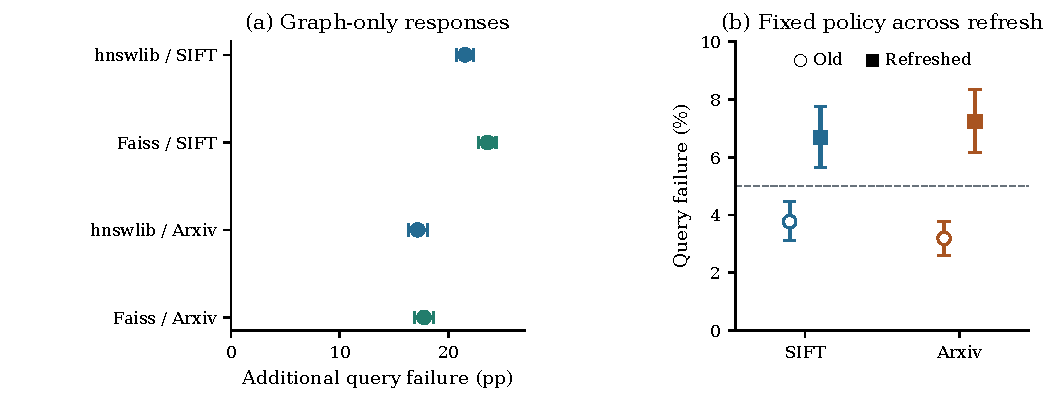
\includegraphics[width=\textwidth]{figures_v3/overview.pdf}
\caption{Two failures that motivate ICBA. Left: graph-only transfer of retrospective first-passing actions, with a query-cluster interval conditional on fixed builds. Right: one executable recurring-query policy before and after a 5\% refresh, with a crossed target-build/query interval.}
\label{fig:overview}
\Description{Four graph-only incremental-risk estimates are positive. In the refresh test, risk increases on both datasets and crosses five percent.}
\end{figure*}

\begin{table}[t]
\caption*{\textbf{Terms at a glance.} Tables shorten Arxiv-Nomic-100K to Arxiv.}
\small\begin{tabularx}{\linewidth}{@{}lX@{}}\toprule
Term & Meaning \\\midrule
ICBA & Audit contract for target portability and deployment.\\
TCP & Target-calibrated pooling for recurring profiled queries.\\
Action & One native search-budget value.\\
Policy & Rule mapping permitted observations to an action.\\
Candidate & Frozen policy/action awaiting certification.\\
Completed decision & Executed candidate, fallback, or abstention.\\
NDC & Number of distance calculations.\\
CP / UCB & Clopper--Pearson / upper confidence bound.\\
LOTO & Leave one target build out.\\
Endpoint & Largest registered native action.\\\bottomrule
\end{tabularx}
\end{table}

We make three contributions. First, we establish budget non-portability across graph-only rebuilds, data refresh, implementations, graph families, and 100K-to-1M scale while retaining each setting's estimand. Second, ICBA supplies a reusable protocol that separates response evidence, target qualification, completed execution, and information cost. Third, a preregistered recovery and baseline program identifies when complexity is warranted: target calibration is beneficial on the registered prospective panels, TCP adds resolved query-conditional value on SIFT, and a simple fixed action can match or outperform a source-tailored heuristic under the common risk contract. The artifact regenerates the paper, validates the decision chain, and preserves query-role boundaries.

The systems implication is direct: version the budget policy with its index and workload; qualify reuse on the target; and escalate from fixed to target-global to query-conditional policies only when the measured gain justifies their information cost.
